% ============================================================================
%  fig_system_overview.tex -- high-level schematic of the proposed pipeline.
%  Sample-thesis Figure-3.1 style: six stages in a two-row snake flow.
%  Colours follow the house palette; the two modifications are red-accented.
%  Needs \usepackage{tikz} (loaded in thesisstyle.sty).
%  Include with:  % ============================================================================
%  fig_system_overview.tex -- high-level schematic of the proposed pipeline.
%  Sample-thesis Figure-3.1 style: six stages in a two-row snake flow.
%  Colours follow the house palette; the two modifications are red-accented.
%  Needs \usepackage{tikz} (loaded in thesisstyle.sty).
%  Include with:  % ============================================================================
%  fig_system_overview.tex -- high-level schematic of the proposed pipeline.
%  Sample-thesis Figure-3.1 style: six stages in a two-row snake flow.
%  Colours follow the house palette; the two modifications are red-accented.
%  Needs \usepackage{tikz} (loaded in thesisstyle.sty).
%  Include with:  % ============================================================================
%  fig_system_overview.tex -- high-level schematic of the proposed pipeline.
%  Sample-thesis Figure-3.1 style: six stages in a two-row snake flow.
%  Colours follow the house palette; the two modifications are red-accented.
%  Needs \usepackage{tikz} (loaded in thesisstyle.sty).
%  Include with:  \input{tikz/fig_system_overview}
% ============================================================================
\definecolor{soBlueFill}{HTML}{DAE8FC}
\definecolor{soBlueStroke}{HTML}{6C8EBF}
\definecolor{soGreenFill}{HTML}{D5E8D4}
\definecolor{soGreenStroke}{HTML}{82B366}
\definecolor{soOrangeFill}{HTML}{FFE6CC}
\definecolor{soOrangeStroke}{HTML}{D79B00}
\definecolor{soPurpleFill}{HTML}{E1D5E7}
\definecolor{soPurpleStroke}{HTML}{9673A6}
\definecolor{soRed}{HTML}{FF0000}
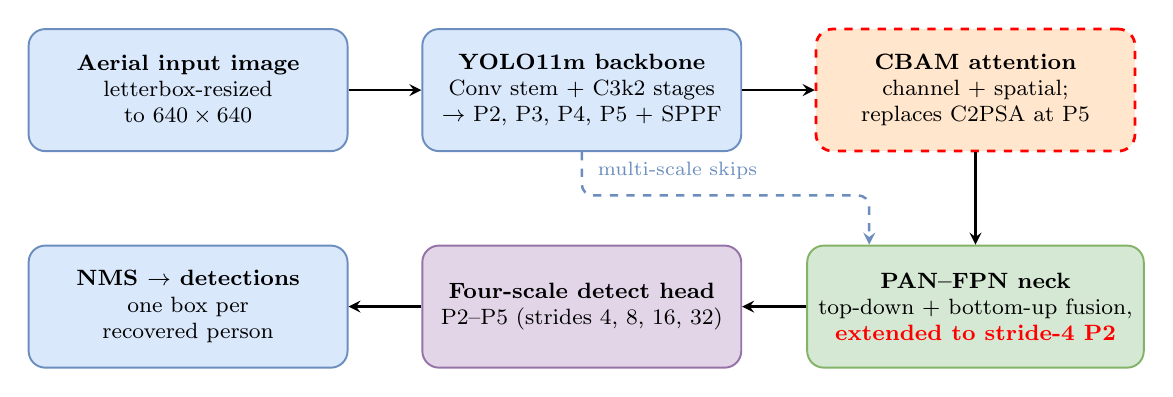
\begin{tikzpicture}[
  font=\footnotesize,
  stage/.style={rounded corners=6pt, draw, align=center,
                minimum width=4.05cm, minimum height=1.55cm,
                inner sep=4pt, line width=0.7pt},
  flow/.style={-{stealth}, line width=0.9pt}
]
  % ---- row 1 (left to right) ----
  \node[stage, fill=soBlueFill, draw=soBlueStroke] (inp) at (0,0)
        {\textbf{Aerial input image}\\letterbox-resized\\to $640\times640$};
  \node[stage, fill=soBlueFill, draw=soBlueStroke] (bb) at (5.0,0)
        {\textbf{YOLO11m backbone}\\Conv stem + C3k2 stages\\$\rightarrow$ P2, P3, P4, P5 + SPPF};
  \node[stage, fill=soOrangeFill, draw=soRed, dashed, line width=1.0pt] (cbam) at (10.0,0)
        {\textbf{CBAM attention}\\channel + spatial;\\replaces C2PSA at P5};

  % ---- row 2 (right to left) ----
  \node[stage, fill=soGreenFill, draw=soGreenStroke] (neck) at (10.0,-2.75)
        {\textbf{PAN--FPN neck}\\top-down + bottom-up fusion,\\\textcolor{soRed}{\textbf{extended to stride-4 P2}}};
  \node[stage, fill=soPurpleFill, draw=soPurpleStroke] (head) at (5.0,-2.75)
        {\textbf{Four-scale detect head}\\P2--P5 (strides 4, 8, 16, 32)};
  \node[stage, fill=soBlueFill, draw=soBlueStroke] (out) at (0,-2.75)
        {\textbf{NMS $\rightarrow$ detections}\\one box per\\recovered person};

  % ---- flow arrows (snake) ----
  \draw[flow] (inp) -- (bb);
  \draw[flow] (bb) -- (cbam);
  \draw[flow] (cbam) -- (neck);
  \draw[flow] (neck) -- (head);
  \draw[flow] (head) -- (out);

  % ---- skip connections annotation (orthogonal, through the row gap) ----
  \draw[flow, dashed, soBlueStroke, rounded corners=4pt]
        (bb.south) -- ++(0,-0.55)
        node[pos=1, above right=2pt, font=\scriptsize, text=soBlueStroke]
        {multi-scale skips}
        -| ([xshift=-1.35cm]neck.north);
\end{tikzpicture}

% ============================================================================
\definecolor{soBlueFill}{HTML}{DAE8FC}
\definecolor{soBlueStroke}{HTML}{6C8EBF}
\definecolor{soGreenFill}{HTML}{D5E8D4}
\definecolor{soGreenStroke}{HTML}{82B366}
\definecolor{soOrangeFill}{HTML}{FFE6CC}
\definecolor{soOrangeStroke}{HTML}{D79B00}
\definecolor{soPurpleFill}{HTML}{E1D5E7}
\definecolor{soPurpleStroke}{HTML}{9673A6}
\definecolor{soRed}{HTML}{FF0000}
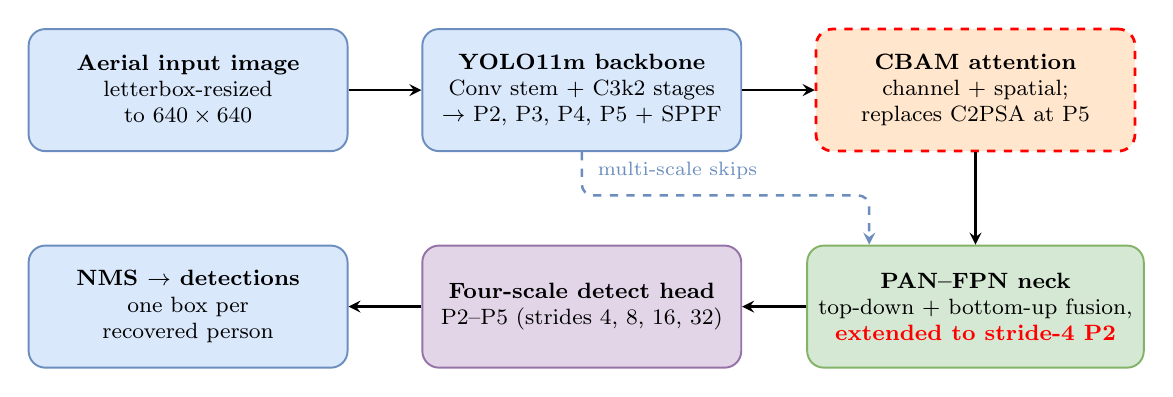
\begin{tikzpicture}[
  font=\footnotesize,
  stage/.style={rounded corners=6pt, draw, align=center,
                minimum width=4.05cm, minimum height=1.55cm,
                inner sep=4pt, line width=0.7pt},
  flow/.style={-{stealth}, line width=0.9pt}
]
  % ---- row 1 (left to right) ----
  \node[stage, fill=soBlueFill, draw=soBlueStroke] (inp) at (0,0)
        {\textbf{Aerial input image}\\letterbox-resized\\to $640\times640$};
  \node[stage, fill=soBlueFill, draw=soBlueStroke] (bb) at (5.0,0)
        {\textbf{YOLO11m backbone}\\Conv stem + C3k2 stages\\$\rightarrow$ P2, P3, P4, P5 + SPPF};
  \node[stage, fill=soOrangeFill, draw=soRed, dashed, line width=1.0pt] (cbam) at (10.0,0)
        {\textbf{CBAM attention}\\channel + spatial;\\replaces C2PSA at P5};

  % ---- row 2 (right to left) ----
  \node[stage, fill=soGreenFill, draw=soGreenStroke] (neck) at (10.0,-2.75)
        {\textbf{PAN--FPN neck}\\top-down + bottom-up fusion,\\\textcolor{soRed}{\textbf{extended to stride-4 P2}}};
  \node[stage, fill=soPurpleFill, draw=soPurpleStroke] (head) at (5.0,-2.75)
        {\textbf{Four-scale detect head}\\P2--P5 (strides 4, 8, 16, 32)};
  \node[stage, fill=soBlueFill, draw=soBlueStroke] (out) at (0,-2.75)
        {\textbf{NMS $\rightarrow$ detections}\\one box per\\recovered person};

  % ---- flow arrows (snake) ----
  \draw[flow] (inp) -- (bb);
  \draw[flow] (bb) -- (cbam);
  \draw[flow] (cbam) -- (neck);
  \draw[flow] (neck) -- (head);
  \draw[flow] (head) -- (out);

  % ---- skip connections annotation (orthogonal, through the row gap) ----
  \draw[flow, dashed, soBlueStroke, rounded corners=4pt]
        (bb.south) -- ++(0,-0.55)
        node[pos=1, above right=2pt, font=\scriptsize, text=soBlueStroke]
        {multi-scale skips}
        -| ([xshift=-1.35cm]neck.north);
\end{tikzpicture}

% ============================================================================
\definecolor{soBlueFill}{HTML}{DAE8FC}
\definecolor{soBlueStroke}{HTML}{6C8EBF}
\definecolor{soGreenFill}{HTML}{D5E8D4}
\definecolor{soGreenStroke}{HTML}{82B366}
\definecolor{soOrangeFill}{HTML}{FFE6CC}
\definecolor{soOrangeStroke}{HTML}{D79B00}
\definecolor{soPurpleFill}{HTML}{E1D5E7}
\definecolor{soPurpleStroke}{HTML}{9673A6}
\definecolor{soRed}{HTML}{FF0000}
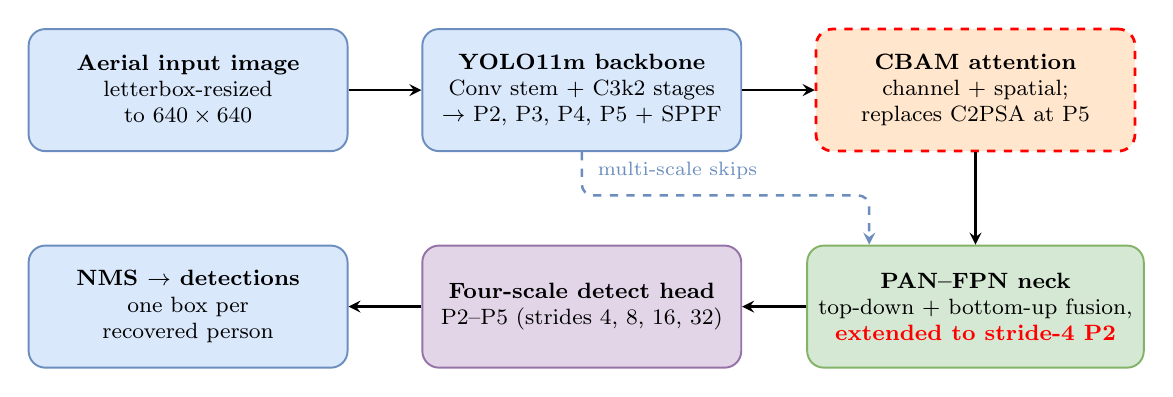
\begin{tikzpicture}[
  font=\footnotesize,
  stage/.style={rounded corners=6pt, draw, align=center,
                minimum width=4.05cm, minimum height=1.55cm,
                inner sep=4pt, line width=0.7pt},
  flow/.style={-{stealth}, line width=0.9pt}
]
  % ---- row 1 (left to right) ----
  \node[stage, fill=soBlueFill, draw=soBlueStroke] (inp) at (0,0)
        {\textbf{Aerial input image}\\letterbox-resized\\to $640\times640$};
  \node[stage, fill=soBlueFill, draw=soBlueStroke] (bb) at (5.0,0)
        {\textbf{YOLO11m backbone}\\Conv stem + C3k2 stages\\$\rightarrow$ P2, P3, P4, P5 + SPPF};
  \node[stage, fill=soOrangeFill, draw=soRed, dashed, line width=1.0pt] (cbam) at (10.0,0)
        {\textbf{CBAM attention}\\channel + spatial;\\replaces C2PSA at P5};

  % ---- row 2 (right to left) ----
  \node[stage, fill=soGreenFill, draw=soGreenStroke] (neck) at (10.0,-2.75)
        {\textbf{PAN--FPN neck}\\top-down + bottom-up fusion,\\\textcolor{soRed}{\textbf{extended to stride-4 P2}}};
  \node[stage, fill=soPurpleFill, draw=soPurpleStroke] (head) at (5.0,-2.75)
        {\textbf{Four-scale detect head}\\P2--P5 (strides 4, 8, 16, 32)};
  \node[stage, fill=soBlueFill, draw=soBlueStroke] (out) at (0,-2.75)
        {\textbf{NMS $\rightarrow$ detections}\\one box per\\recovered person};

  % ---- flow arrows (snake) ----
  \draw[flow] (inp) -- (bb);
  \draw[flow] (bb) -- (cbam);
  \draw[flow] (cbam) -- (neck);
  \draw[flow] (neck) -- (head);
  \draw[flow] (head) -- (out);

  % ---- skip connections annotation (orthogonal, through the row gap) ----
  \draw[flow, dashed, soBlueStroke, rounded corners=4pt]
        (bb.south) -- ++(0,-0.55)
        node[pos=1, above right=2pt, font=\scriptsize, text=soBlueStroke]
        {multi-scale skips}
        -| ([xshift=-1.35cm]neck.north);
\end{tikzpicture}

% ============================================================================
\definecolor{soBlueFill}{HTML}{DAE8FC}
\definecolor{soBlueStroke}{HTML}{6C8EBF}
\definecolor{soGreenFill}{HTML}{D5E8D4}
\definecolor{soGreenStroke}{HTML}{82B366}
\definecolor{soOrangeFill}{HTML}{FFE6CC}
\definecolor{soOrangeStroke}{HTML}{D79B00}
\definecolor{soPurpleFill}{HTML}{E1D5E7}
\definecolor{soPurpleStroke}{HTML}{9673A6}
\definecolor{soRed}{HTML}{FF0000}
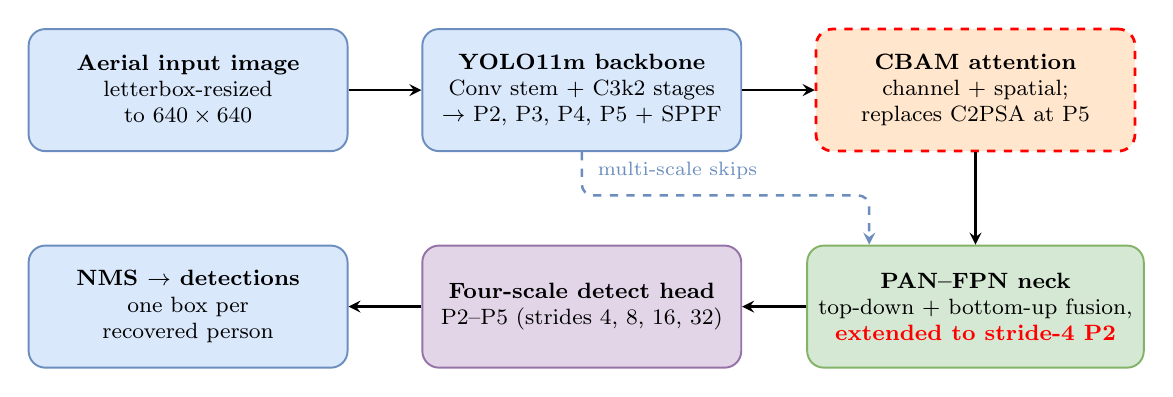
\begin{tikzpicture}[
  font=\footnotesize,
  stage/.style={rounded corners=6pt, draw, align=center,
                minimum width=4.05cm, minimum height=1.55cm,
                inner sep=4pt, line width=0.7pt},
  flow/.style={-{stealth}, line width=0.9pt}
]
  % ---- row 1 (left to right) ----
  \node[stage, fill=soBlueFill, draw=soBlueStroke] (inp) at (0,0)
        {\textbf{Aerial input image}\\letterbox-resized\\to $640\times640$};
  \node[stage, fill=soBlueFill, draw=soBlueStroke] (bb) at (5.0,0)
        {\textbf{YOLO11m backbone}\\Conv stem + C3k2 stages\\$\rightarrow$ P2, P3, P4, P5 + SPPF};
  \node[stage, fill=soOrangeFill, draw=soRed, dashed, line width=1.0pt] (cbam) at (10.0,0)
        {\textbf{CBAM attention}\\channel + spatial;\\replaces C2PSA at P5};

  % ---- row 2 (right to left) ----
  \node[stage, fill=soGreenFill, draw=soGreenStroke] (neck) at (10.0,-2.75)
        {\textbf{PAN--FPN neck}\\top-down + bottom-up fusion,\\\textcolor{soRed}{\textbf{extended to stride-4 P2}}};
  \node[stage, fill=soPurpleFill, draw=soPurpleStroke] (head) at (5.0,-2.75)
        {\textbf{Four-scale detect head}\\P2--P5 (strides 4, 8, 16, 32)};
  \node[stage, fill=soBlueFill, draw=soBlueStroke] (out) at (0,-2.75)
        {\textbf{NMS $\rightarrow$ detections}\\one box per\\recovered person};

  % ---- flow arrows (snake) ----
  \draw[flow] (inp) -- (bb);
  \draw[flow] (bb) -- (cbam);
  \draw[flow] (cbam) -- (neck);
  \draw[flow] (neck) -- (head);
  \draw[flow] (head) -- (out);

  % ---- skip connections annotation (orthogonal, through the row gap) ----
  \draw[flow, dashed, soBlueStroke, rounded corners=4pt]
        (bb.south) -- ++(0,-0.55)
        node[pos=1, above right=2pt, font=\scriptsize, text=soBlueStroke]
        {multi-scale skips}
        -| ([xshift=-1.35cm]neck.north);
\end{tikzpicture}
